\chapter{Noțiuni teoretice}

\section{Rețele Neurale Recurente}

Rețelele neuronale recurente (RNN - Recurent Neural Networks), sunt o arhitectura aparte de rețele neuronale, ce le face atat de speciale este faptul ca ele reușesc sa capteze secvențialitatea datelor. Ele sunt folosite in special în procesarea limbajului natural, dar și în procesarea imaginilor, a seriilor de timp, a recomandarilor de produse. Cu alte cuvinte oricând vine vorba de succesiunea anumitor evenimente, ele reprezintă un candidat bun în captarea acestor modele in date.

Figura \ref{fig:rnn_arch} prezintă arhitectura unei rețele recurente, unde fiecare dreptunghi ține locul stratului ascuns de la pasul, $t$. Fiecare strat ascuns este format din perceptroni care execută operația de inmulțire intre parametrii și input, urmată de o operație nonlineară (ex.$ tanh$). La fiecare pas din timp, ieșirea de la pasul anterior, împreună cu vectorul următorului cuvânt, $x_t$, sunt intrări în stratul ascuns care produce pentru pasul următor, iețirea $y$, și vectorul de caracteristici al stratului ascuns, $h$.


$$h_t = \sigma{(W^{(hh)} h_{t-1} + W^{(hx)} x_{[t]})}$$
$$y = softmax(W^{(S)} h_t)$$


\begin{figure}[h]
	\centering
	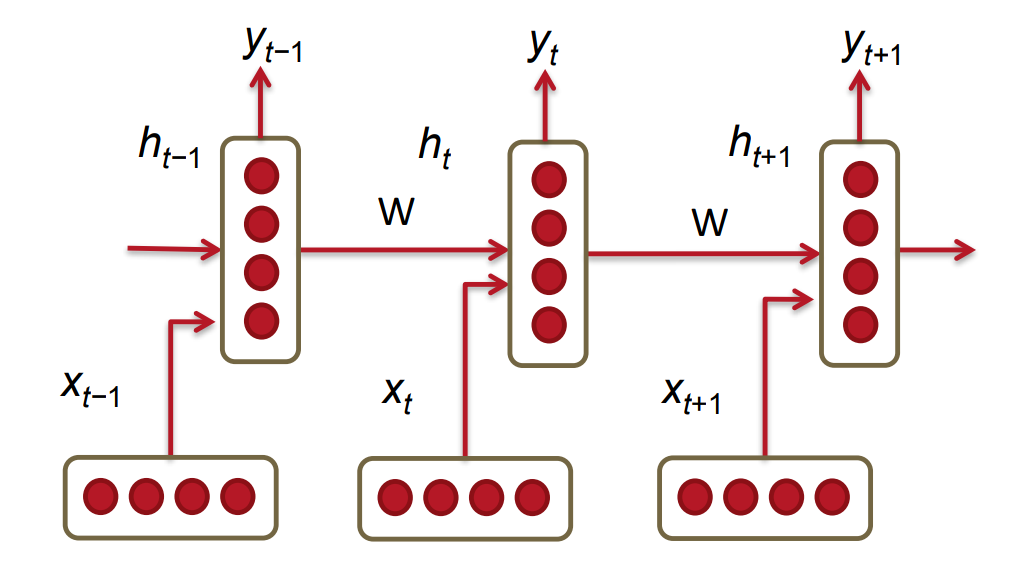
\includegraphics[scale=0.3]{rnn_arch.png}
	\caption{Arhitectura RNN \cite{cs224d_notes}}
	\label{fig:rnn_arch}
\end{figure}

Descrierea parametrilor din rețea:

\begin{itemize}
	\item $x_1, x_2, ..., x_T$ vectorii cuvintelor dintr-o secvență de lungime $T$
	\item $h_t = \sigma{(W^{(hh)} h_{t-1} + W^{(hx)} x_{[t]})}$: formula care descrie calculul vectorului de caracteristici, $h_t$, la fiecare pas $t$:
	
	\begin{itemize}
		\item $x_t \in {\rm I\!R}^d$ vectorul cuvântului $t$
		 
	\end{itemize}
\end{itemize}


\cite{cs224d_notes}

\subsection{LSTM}



\subsection{Seq2Seq}